%
% Template Laporan Tugas Akhir Jurusan Informatika Unsyiah 
%
% @author Abdul Hafidh
% @version 1.1
% @since 08.09.2023
%
% Template ini telah disesuaikan dengan aturan penulisan tugas akhir yang terdapat pada dokumen Panduan Tugas Akhir FMIPA Unsyiah tahun 2016.
%


% karena jifhasiltheme.cls ada di folder lib, maka kita harus menambahkan path lib/ ke dalam path pencarian file
\makeatletter
\def\input@path{{lib/}}
\makeatother
% Template pembuatan naskah tugas akhir.
\documentclass[dvipsnames]{jifproposal-abdul}






\tolerance=1
\emergencystretch=\maxdimen
\hyphenpenalty=10000
\hbadness=10000

%\usepackage[a4paper,left=14cm,right=3cm,top=3cm,bottom=5cm]{geometry}
%karena file hype.indonesia.tex ada di folder language, maka kita harus menambahkan path language/ ke dalam path pencarian file
\makeatletter
\def\input@path{{language/}}
\makeatother
% Daftar pemenggalan suku kata dan istilah dalam LaTeX
%
% Hyphenation untuk Indonesia 
%
% @author  Andreas Febrian
% @version 1.00
% 
% Tambahkan cara pemenggalan kata-kata yang salah dipenggal secara otomatis 
% oleh LaTeX. Jika kata tersebut dapat dipenggal dengan benar, maka tidak 
% perlu ditambahkan dalam berkas ini. Tanda pemenggalan kata menggunakan 
% tanda '-'; contoh:
% menarik
%   --> pemenggalan: me-na-rik
%

\hyphenation{
    % alphabhet A
    a-na-li-sa a-tur 
    a-pli-ka-si 
    android
    % alphabhet B
    ba-ngun-an 
    be-be-ra-pa 
    ber-ge-rak
    ber-ke-lan-jut-an 
    ber-pe-nga-ruh 
    % alphabhet C
    ca-ri
    % alphabhet D
    di-sim-pan di-pim-pin de-ngan da-e-rah di-ba-ngun da-pat di-nya-ta-kan 
    di-sim-bol-kan di-pi-lih di-li-hat de-fi-ni-si
    % alphabhet E
    e-ner-gi eks-klu-sif
    % alphabhet F
    fa-si-li-tas
    foot-print
    % alphabhet G
    ga-bung-an ge-rak
    % alphabhet H
    ha-lang-an
    % alphabhet I
    % alphabhet J
    % alphabhet K
    ke-hi-lang-an
    ku-ning 
    kua-li-tas ka-me-ra ke-mung-kin-an ke-se-pa-ham-an
    % alphabhet L
    ling-kung-an
    % alphabhet M
    me-neng-ah
    meng-a-tas-i me-mung-kin-kan me-nge-na-i me-ngi-rim-kan 
    meng-u-bah meng-a-dap-ta-si me-nya-ta-kan mo-di-fi-ka-si
    meng-a-tur
    mem-pro-mo-si-kan
    me-la-ku-kan
    meng-i-den-ti-fi-ka-si-kan
    % alphabhet N
    nya-ta non-eks-klu-sif
    % alphabhet O
    % alphabhet P
	pe-nye-rap-an 
	pe-ngon-trol
    pe-mo-del-an
    pe-ran  pe-ran-an-nya
    pem-ba-ngun-an pre-si-den pe-me-rin-tah prio-ri-tas peng-am-bil-an 
    peng-ga-bung-an pe-nga-was-an pe-ngem-bang-an 
    pe-nga-ruh pa-ra-lel-is-me per-hi-tung-an per-ma-sa-lah-an 
    pen-ca-ri-an peng-struk-tur-an
    pe-ran-ca-ngan
    plat-form
    patch
    % alphabhet Q
    % alphabhet R
    ran-cang-an
    % alphabhet S
    si-mu-la-si sa-ngat
    smart-phone
    % alphabhet T
    te-ngah
    ter-da-pat
    % alphabhet U
    % alphabhet V
    % alphabhet W
    % alphabhet X
    % alphabhet Y
    % alphabhet Z
    % special
}

% Untuk prefiks pada daftar gambar dan tabel
\usepackage[titles]{tocloft}

\usepackage{etoolbox}% http://ctan.org/pkg/etoolbox
\makeatletter
% \patchcmd{<cmd>}{<search>}{<replace>}{<succes>}{<failure>}
\patchcmd{\@chapter}{\addtocontents{lof}{\protect\addvspace{10\p@}}}{}{}{}% LoF
\patchcmd{\@chapter}{\addtocontents{lot}{\protect\addvspace{10\p@}}}{}{}{}% LoT
\makeatother




\usepackage{titlesec}

\usepackage[justification=centering]{caption}% or e.g. [format=hang]

% Ini tambahan dari budi
\newcommand*{\enableboldchapterintoc}{%
  \addtocontents{toc}{\string\renewcommand{\protect\cftchapfont}{\protect\normalfont\protect\bfseries}}
  \addtocontents{toc}{\string\renewcommand{\protect\cftchappagefont}{\protect\normalfont\protect}}
  \addtocontents{toc}{\protect\setlength{\cftbeforechapskip}{12pt}}
}
\newcommand*{\disableboldchapterintoc}{%
  \addtocontents{toc}{\string\renewcommand{\protect\cftchappagefont}{\protect\normalfont}}
  \addtocontents{toc}{\string\renewcommand{\protect\cftchapfont}{\protect\normalfont}}
  \addtocontents{toc}{\protect\setlength{\cftbeforechapskip}{0pt}}
}
% Ini tambahan dari budi

\renewcommand{\cftdotsep}{0.5}
\renewcommand{\cftchapleader}{\cftdotfill{\cftdotsep}}
%\renewcommand{\cftpartleader}{\cftdotfill{\cftdotsep}}

\renewcommand\cftfigpresnum{Gambar\  }
\renewcommand\cfttabpresnum{Tabel\   }

% \newcommand{\listappendicesname}{DAFTAR LAMPIRAN}
%\newlistof{appendices}{apc}{\listappendicesname}
\newcommand{\appendices}[1]{\addcontentsline{apc}{appendices}{#1}}
\newcommand{\newappendix}[1]{\section*{#1}\appendices{#1}}

% Untuk hyperlink dan table of content
\usepackage[hidelinks]{hyperref}
\renewcommand\UrlFont{\rmfamily\itshape} %it's me!
\newlength{\mylenf}
\settowidth{\mylenf}{\cftfigpresnum}
\setlength{\cftfignumwidth}{\dimexpr\mylenf+2em}
\setlength{\cfttabnumwidth}{\dimexpr\mylenf+2em}
% prevent

% Agar ada tulisan BAB pada TOC
\renewcommand\cftchappresnum{BAB } 
  \cftsetindents{chapter}{0em}{4.5em} %indenting bab
  \cftsetindents{section}{4.5em}{2em}
  \cftsetindents{subsection}{6.5em}{3em}
 
% Agar di TOC setiap angka bab/subbab diakhiri titik

\renewcommand{\cftsecaftersnum}{.}
\renewcommand{\cftsubsecaftersnum}{.}

% Agar setiap angka bab/subbab diakhiri titik
\usepackage{titlesec}
\titlelabel{\thetitle.\quad}

% Agar disetiap caption table dan gambar diakhiri titik
\usepackage[labelsep=period]{caption}

% Untuk Bold Face pada Keterangan Gambar
\usepackage[labelfont=bf]{caption}

% Untuk caption dan subcaption
\usepackage{caption}
\usepackage{subcaption}


% Agar bisa menggunakan warna LaTeX
\usepackage{color} %it's me!

% Agar table yang panjang bisa cut ke next page    %byRennyAdr
\usepackage{longtable}

% Untuk page landscape        %byRennyAdr
\usepackage{pdflscape}
\usepackage{lscape}

% Agar bisa bikin code snippet
\usepackage{listings, lstautogobble} %it's me!

\usepackage{adjustbox}

% untuk shadow gambar     %tomy
\usepackage{fancybox, graphicx}

% untuk cite url
\usepackage{url}
\usepackage{microtype} % untuk mengatur spasi pada paragraf

\usepackage{siunitx}

\usepackage{xcolor}
\usepackage{multirow}
\usepackage[normalem]{ulem}
\useunder{\uline}{\ul}{}

\usepackage{array}
\newcolumntype{P}[1]{>{\centering\arraybackslash}p{#1}}
\newcolumntype{M}[1]{>{\centering\arraybackslash}m{#1}}


\makeatletter
\def\input@path{{include/}}
\makeatother
% Sampul Depan
%-----------------------------------------------------------------
% Sampul Depan
%-----------------------------------------------------------------
\judulcover{LOREM IPSUM DOLOR SI AMET}

\judul{LOREM IPSUM DOLOR SI AMET}

\judulinggris{LOREM IPSUM DOLOR SI AMET}

% nama lengkap
\fullname{Anton }

% NPM (Nomor Pokok Mahasiswa)
\idnum{2134312432134}

\degree{Sarjana Komputer}

\yearsubmit{Januari, 2024}

\program{Informatika}

\dept{Informatika}

% Pembimbing Pertama
\firstsupervisor{<pembimbing1>}
\firstnip{<nip pembimbing1}

% Pembimbing Kedua
\secondsupervisor{<pembimbing 2>}
\secondnip{<nip pembimbing 2>}

% Ketua Jurusan
\kajur{Viska Mutiawani, B.IT, M.IT.}
\kajurnip{198008312009122003}

% Dekan Fakultas
\dekan{Prof. Dr. Teuku M. Iqbalsyah, S.Si, M.Sc.}
\dekannip{197110101997031003}
% Dekan Fakultas
%\dekan{Dr. Teuku Mohamad Iqbalsyah, S.Si., M.Sc.}
%\dekannip{197110101997031003}

%kaprodi
\kaprodi{Viska Mutiawani, B.IT, M.IT.}
\kaprodinip{198008312009122003}

% tangal lulus proposal, seminar hasil atau sidang
\approvaldate{Kamis, 14 Mei 2024}

%-----------------------------------------------------------------
% End of Sampul Depan
%-----------------------------------------------------------------


% Awal dokumen
\usepackage{fancyhdr}
\usepackage{rotating}
% Untuk prefiks pada Daftar Program   
% byRennyAdr
\makeatletter
\begingroup\let\newcounter\@gobble\let\setcounter\@gobbletwo
\globaldefs\@ne \let\c@loldepth\@ne
\newlistof{listings}{lol}{\lstlistlistingname}
\endgroup
\let\l@lstlisting\l@listings
\AtBeginDocument{\addtocontents{lol}{\protect\addvspace{10\p@}}}
\makeatother
\renewcommand{\lstlistoflistings}{\listoflistings}
\renewcommand\cftlistingspresnum{Program~}
\cftsetindents{listings}{1.5em}{7em}

%tab didaftar pustaka -Indah
\setlength{\bibhang}{30pt}


%split rumus -Indah
\usepackage{amsmath}



\begin{document}
\fancyhf{} 
\fancyfoot[R]{\thepage}


\cover
\include{daftar-singkatan} % jangan dihapus



 %berikan comment jika proposal


%-----------------------------------------------------------------
% TOC menggunakan single space
%-----------------------------------------------------------------



\addcontentsline{toc}{chapter}{Daftar Isi}

\begin{singlespace}
	\tableofcontents
\end{singlespace}
\listoftables
\addcontentsline{toc}{chapter}{Daftar Tabel}
\listoffigures
\addcontentsline{toc}{chapter}{Daftar Gambar}




\listofappendices

\enableboldchapterintoc
%-----------------------------------------------------------------
% Daftar Singkatan 
%-----------------------------------------------------------------
\include{daftar-singkatan} % jangan dihapus

% Caption untuk code snippet. it's me!
\renewcommand{\thelstlisting}{\arabic{chapter}.\arabic{lstlisting}}
\renewcommand*\lstlistingname{Program}

%-----------------------------------------------------------------
% Disini awal masukan untuk Bab
%-----------------------------------------------------------------
\begin{onehalfspace}

\fancyhf{} 
\fancyfoot[C]{\thepage}
\pagenumbering{arabic}

\captionsetup[figure]{labelfont={normalfont}, textfont={normalfont}} % Unbold caption gambar
\captionsetup[table]{labelfont={normalfont}, textfont={normalfont}} % Unbold caption tabel

% \fancyhf{} 
% \fancyfoot[R]{\thepage}

\chapter{PENDAHULUAN}
%\thispagestyle{plain} % Halaman pertama bab menggunakan gaya plain

\section{Latar Belakang}
% Menambahkan lorem ipsum
Lorem ipsum dolor sit amet, consectetur adipiscing elit. Sed euismod, nisl quis lacinia ultricies, nunc nisl ultricies diam, quis aliqua \citep{WHO2020}


\section{Rumusan Masalah}
Berdasarkan latar belakang di atas, permasalahan dalam penelitian ini dapat dirumuskan sebagai berikut:
\begin{enumerate}
	\item lorem ipsum dolor sit amet, consectetur adipiscing elit. Sed euismod, nisl quis lacinia ultricies,
	\item lorem ipsum dolor sit amet, consectetur adipiscing elit. Sed euismod, nisl quis lacinia ultricies,
	\item lorem ipsum dolor sit amet, consectetur adipiscing elit. Sed euismod, nisl quis lacinia ultricies,
	\item lorem ipsum dolor sit amet, consectetur adipiscing elit. Sed euismod, nisl quis lacinia ultricies,
\end{enumerate}

\section{Tujuan Penelitian}
Berdasarkan rumusan masalah yang telah disebutkan sebelumnya, maka dapat dipaparkan tujuan dari penelitian ini adalah sebagai berikut:
\begin{enumerate}
	\item lorem ipsum dolor sit amet, consectetur adipiscing elit. Sed euismod, nisl quis lacinia ultricies,
	\item lorem ipsum dolor sit amet, consectetur adipiscing elit. Sed euismod, nisl quis lacinia ultricies,
	\item lorem ipsum dolor sit amet, consectetur adipiscing elit. Sed euismod, nisl quis lacinia ultricies,
	\item lorem ipsum dolor sit amet, consectetur adipiscing elit. Sed euismod, nisl quis lacinia ultricies,
\end{enumerate}


\section{Manfaat Penelitian}
Adapun manfaat dari penelitian ini adalah sebagai berikut:
\begin{enumerate}
	\item lorem ipsum dolor sit amet, consectetur adipiscing elit. Sed euismod, nisl quis lacinia ultricies,
	\item lorem ipsum dolor sit amet, consectetur adipiscing elit. Sed euismod, nisl quis lacinia ultricies,
	\item lorem ipsum dolor sit amet, consectetur adipiscing elit. Sed euismod, nisl quis lacinia ultricies,
	\item lorem ipsum dolor sit amet, consectetur adipiscing elit. Sed euismod, nisl quis lacinia ultricies,

\end{enumerate}



% Baris ini digunakan untuk membantu dalam melakukan sitasi
% Karena diapit dengan comment, maka baris ini akan diabaikan
% oleh compiler LaTeX.
\begin{comment}
\bibliography{daftar-pustaka}
\end{comment}


%-------------------------------------------------------------------------------
%                            BAB II
%               TINJAUAN PUSTAKA DAN DASAR TEORI
%-------------------------------------------------------------------------------
\fancyhf{} 
\fancyfoot[R]{\thepage}
\chapter{TINJAUAN PUSTAKA}

\par Untuk mendukung penelitian ini, maka dalam bab ini akan dikemukakan beberapa rumusan teori pendukung yang dikutip dari berbagai referensi baik dalam bentuk buku, artikel, maupun tulisan karya ilmiah lainnya termasuk hasil penelitian sebelumnya yang ada kaitannya dengan penelitian yang dilakukan.
\section{Landasan Teori}
%\subsection{System Usability Scale (SUS)}	
%\par \textit{System Usability Scale} (SUS) dikembangkan oleh \citep{brooke1996} sebagai sebuah pengukuran usability yang \textit{quick and dirty}. SUS menggunakan survei yang terdiri dari 10 pertanyaan, masing-masing memiliki 5 poin Likert sebagai tanggapan, output dari SUS berupa skor yang tampak mudah dipahami, dengan \textit{range} dari 0 hingga 100. Semakin besar skor berarti semakin baik \textit{usability}-nya. 

% \par Pengujian ini memerlukan kuesioner sebagai teknik pengumpulan informasi pengujian yang didapat dari responden mengenai aplikasi. Kuesioner terdiri dari 10 pertanyaan yang terdiri dari pertanyaan positif dan negatif. Pertanyaan positif terdapat pada nomor ganjil (1, 3, 5, 7, 9) dan pertanyaan negatif terdapat pada nomor genap (2, 4, 6, 8, 10). Setiap pertanyaan diberi bobot antara 0 - 4. Pertanyaan ganjil skor dihitung dengan cara bobot tiap pertanyaan (x\textsubscript{i}) dikurangi 1 (ditulis dengan x\textsubscript{i} - 1). Sedangkan pertanyaan genap skor dihitung dengan cara 5 dikurangi bobot tiap pertanyaan (x\textsubscript{i}) (ditulis dengan 5 - x\textsubscript{i}) \citep{ardiansyah2016}.

%-----------------------------------------------------------------------------%

% Baris ini digunakan untuk membantu dalam melakukan sitasi
% Karena diapit dengan comment, maka baris ini akan diabaikan
% oleh compiler LaTeX.

\section{Arsitektur FaceNet}
\par \textit{FaceNet} merupakan \textit{Convolutional Neural Network} (CNN) yang digunakan untuk pengenalan wajah, dikembangkan oleh peneliti dari Google dan dikenalkan pada tahun 2015 \citep{jose2019}. \textit{FaceNet} digunakan untuk mengekstraksi fitur dari gambar wajah seseorang. \textit{FaceNet} mengekstrak wajah menjadi vektor menggunakan \textit{deep} CNN. Vektor nilai atau \textit{vector embedding} yang dihasilkan dapat memetakan kemiripan wajah yang memiliki kedekatan posisi pada \textit{embedding space} \citep{rajagede2021}.

% Menambahkan gambar 
\begin{figure}[H]
\centering
\frame{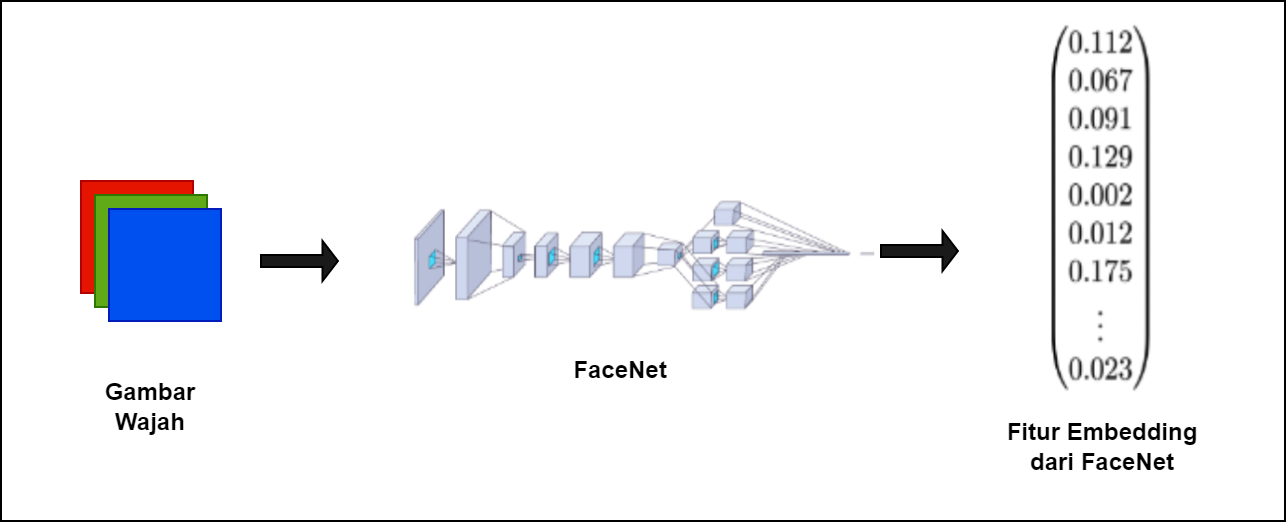
\includegraphics [width = 14cm, height= 5cm]{image/diagram_facenet}}
\caption{\textit{Desain} Arsitektur \textit{FaceNet}}.
\label{dig_facenet}
\end{figure}

\begin{figure}[H]
\centering
\frame{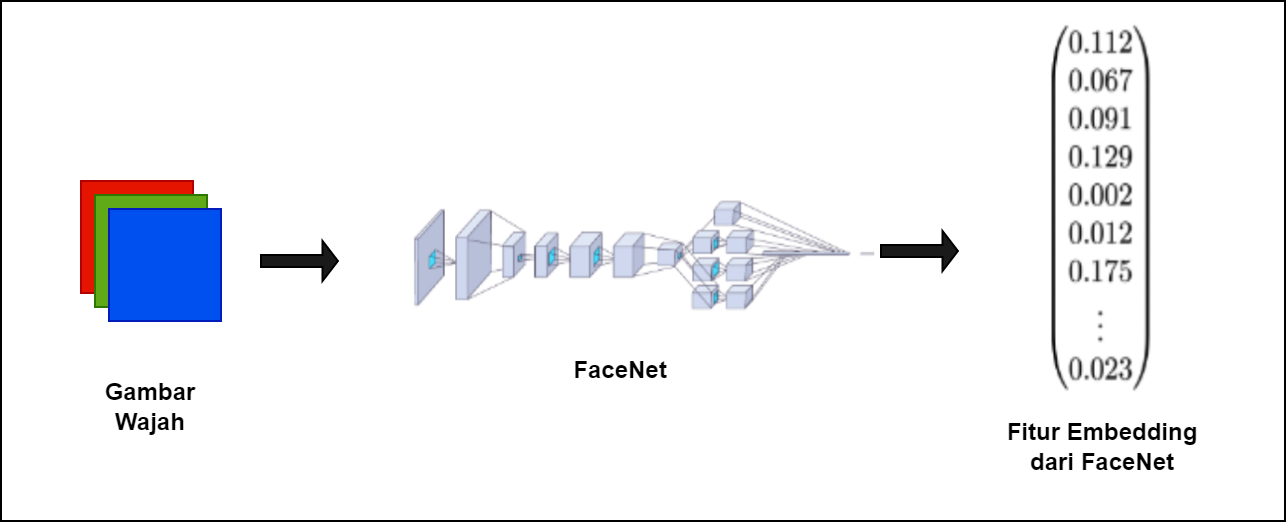
\includegraphics [width = 14cm, height= 5cm]{image/diagram_facenet}}
\caption{\textit{Desain} Arsitektur \textit{FaceNet}}.
\label{dig_facenet}
\end{figure}

\fancyhf{} 
\fancyfoot[R]{\thepage}

\begin{comment}
\bibliography{daftar-pustaka}
\end{comment}


%-------------------------------------------------------------------------------
%                            BAB III
%               		METODOLOGI PENELITIAN
%-------------------------------------------------------------------------------
% \fancyhf{} 
% \fancyfoot[R]{\thepage}
\chapter{METODE PENENILITIAN}
\thispagestyle{plain} % Halaman pertama bab menggunakan gaya plain
\section{Waktu dan Lokasi Penelitian}
Penelitian ini akan bertempat pada beberapa ruangan yang digunakan oleh mahasiswa Jurusan Informatika USK yang umumnya terletak pada lantai 3 blok A dan blok E Gedung Fakultas MIPA USK. Waktu yang dibutuhkan agar penelitian ini dapat di implementasikan adalah 4 bulan terhitung dari bulan Januari 2024 hingga Mei 2024.

\section{Alat dan Bahan}
Alat dan Bahan yang akan digunakan pada penelitian ini terdiri dari beberapa perangkat keras (\textit{hardware}) dan perangkat lunak (\textit{software}) yang dijabarkan sebagai berikut:

\begin{enumerate}
\item Perangkat Keras
	\begin{itemize}
	\item Laptop Lenovo Yoga C740 dengan RAM 16GB DDR4, Intel® Core™ i7-10710U. 1.10 - 4.70 GHz,\textit{Solid State State Drive} (SSD) 1TB.
	\end{itemize}

\item Perangkat Lunak
	\begin{itemize}
	\item Linux Debian Ubuntu 22.04 LTS
	\item Visual Studio Code 1.71.0
	\item Python 3.8.17
	\end{itemize}
\end{enumerate}
\newpage
\section{Metode Penelitian}
Metode penelitian yang dilakukan akan terdiri dari beberapa tahapan penelitian. Skema dari alur tahapan tersebut dapat dilihat pada Gambar \ref{alur_penelitian}.

\begin{figure}[H]
	\centering
	\frame{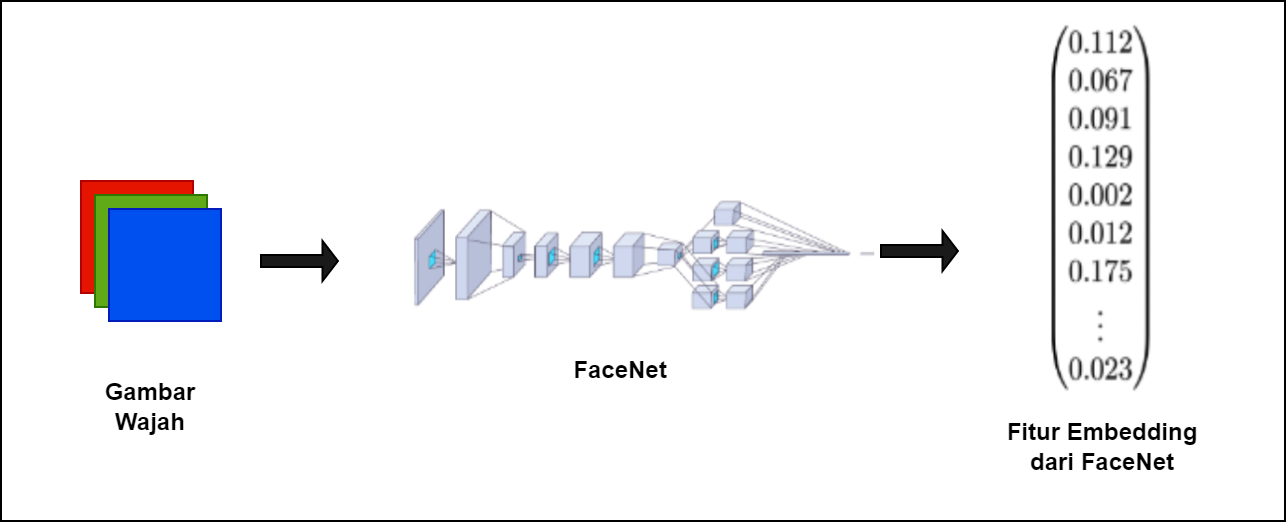
\includegraphics [width = 14cm, height= 5cm]{image/diagram_facenet}}
	\caption{\textit{Desain} Arsitektur \textit{FaceNet}}.
	\label{alur-penelitian} % cuman gambar dummy ya !
\end{figure}

%-----------------------------------------------------------------------------%

% Baris ini digunakan untuk membantu dalam melakukan sitasi
% Karena diapit dengan comment, maka baris ini akan diabaikan
% oleh compiler LaTeX.
\begin{comment}
\bibliography{daftar-pustaka}
\end{comment}

% %-------------------------------------------------------------------------------
%                            BAB IV
%               		HASIL DAN PEMBAHASAN
%-------------------------------------------------------------------------------
% \fancyhf{} 
% \fancyfoot[R]{\thepage}
\chapter{HASIL DAN PEMBAHASAN}
\thispagestyle{plain} % Halaman pertama bab menggunakan gaya plain


\begin{table}[H]
    \centering
    \caption{Hasil Pengujian Akurasi Menggunakan SVM Terhadap Data \textit{Training} dan \textit{Testing}}
    \label{tb_detail_akurasi_face}
    \begin{tabular}{|c|c|c|c|}
    \hline
    \textbf{Jenis Data} & \textbf{Jumlah Label} & \textbf{Jumlah Data} & {\color[HTML]{000000} \textbf{Akurasi}} \\ \hline
    {\color[HTML]{000000} Training} & {\color[HTML]{000000} 41} & {\color[HTML]{000000} 1640} & {\color[HTML]{000000} 99,51\%} \\ \hline
    {\color[HTML]{000000} Testing} & {\color[HTML]{000000} 41} & {\color[HTML]{000000} 410} & {\color[HTML]{000000} 96,34\%} \\ \hline
    \end{tabular}
    \end{table}

% Baris ini digunakan untuk membantu dalam melakukan sitasi
% Karena diapit dengan comment, maka baris ini akan diabaikan
% oleh compiler LaTeX.
\begin{comment}
\bibliography{daftar-pustaka}
\end{comment}

% %-------------------------------------------------------------------------------
%                            BAB V
%               		KESIMPULAN DAN SARAN
%-------------------------------------------------------------------------------
\fancyhf{} 
\fancyfoot[R]{\thepage}
\chapter{KESIMPULAN DAN SARAN}

\section{Kesimpulan}

\section{Saran}


%-----------------------------------------------------------------------------%

% Baris ini digunakan untuk membantu dalam melakukan sitasi
% Karena diapit dengan comment, maka baris ini akan diabaikan
% oleh compiler LaTeX.
\begin{comment}
\bibliography{daftar-pustaka}
\end{comment}

\begin{spacing}{1}
\bibliography{daftar-pustaka}
\end{spacing}
\addcontentsline{toc}{chapter}{DAFTAR PUSTAKA}


%-----------------------------------------------------------------
% Disini akhir masukan Daftar Pustaka
%-----------------------------------------------------------------

%%
% @author Kurnia Saputra
% @version 1.0
% 
% Hanya sebuah pembatas bertuliskan LAMPIRAN ditengah halaman. 
% 

\begin{titlepage}
	\centering 
	\vspace*{6cm}
	\noindent \Huge{LAMPIRAN}
	%\addChapter{LAMPIRAN}
	\addcontentsline{toc}{chapter}{LAMPIRAN}
\end{titlepage}
% \addcontentsline{toc}{chapter}{LAMPIRAN}
\chapter*{LAMPIRAN}
\thispagestyle{plain} % Halaman pertama bab menggunakan gaya plain
% \addcontentsline{toc}{chapter}{LAMPIRAN} %daftar lampiran

\end{onehalfspace}

\end{document}